\chapter{Pipeline}
\label{sec:pipeline}

Como cierre para el proyecto, se ha desarrollado un pipeline capaz de aplicar, al audio recibido como entrada, todos los modelos de IA y XAI explicados en el capítulo de \nameref{sec:metodologia}. Este pipeline tiene como objetivo reunir en un único ``notebook'' todos los modelos desarrollados a lo largo del proyecto. De este modo, permite facilitar la comparación de resultados y explicaciones entre modelos.

Cabe mencionar que el diseño de este pipeline constituye una de las aportaciones prácticas del proyecto, al integrar en una misma estructura modelos de distinta naturaleza y técnicas de explicabilidad complementarias. Esto permite analizar un mismo audio desde múltiples perspectivas, comparando no solo el resultado de clasificación, sino también la forma en que cada modelo justifica su decisión.

Con el fin de representar su estructura general, se ha diseñado un diagrama de flujo simplificado. Como se puede observar en la \autoref{fig:Arquitectura_pipeline}, los modelos se han dividido en dos grupos según el tipo de entrada que utilizan: por un lado, aquellos que operan sobre características extraídas del audio y, por otro, los que trabajan directamente con la forma de onda cruda. En cada grupo se indican tanto los modelos implementados como las técnicas de XAI aplicadas a cada uno de ellos.
\begin{figure}
    \centering
	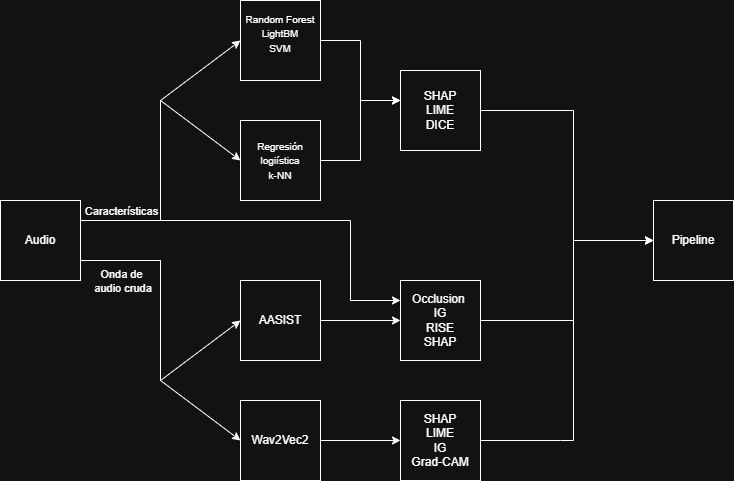
\includegraphics[width=\textwidth]{imagenes/Arquitectura_pipeline.png}
	\caption{Arquitectura del pipeline.}
    \label{fig:Arquitectura_pipeline}
\end{figure}

Para poder reutilizar los modelos entrenados durante el proyecto y evitar su reentrenamiento para cada caso, hemos empleado distintas técnicas para guardarlos. Los modelos que se entrenan con datos tabulares se han guardado mediante la librería joblib y su método \emph{to\_pkl()}, el cual guarda los pesos de los modelos y permite cargarlos fácilmente desde otro archivo. Sobre la forma de guardar el resto de modelos, se explicará en el apartado correspondiente a cada modelo.

La primera parte del ``notebook'' consta de una celda inicial con los imports necesarios, una segunda celda donde se especifica la ruta del audio que se quiere analizar y una tercera celda en la que se extraen las características del audio mediante la función ``\texttt{extract\_features}'' definida en el archivo funciones.py. A partir de ahí, cada modelo tiene su propia sección, en la que se muestra tanto la predicción como las explicaciones obtenidas con las técnicas de XAI asociadas a dicho modelo.

Además, el ``notebook'' está organizado en secciones correspondientes a cada modelo, lo que permite ejecutar cada uno de ellos de forma independiente.

\section{AASIST}

Para poder usar el modelo, lo primero ha sido guardarlo con la función torch.save(). Hemos usado esta función porque nos permite, no solo guardar el modelo para calcular la predicción final, sino también guardar la capa ``sinc-convolution'' para poder aplicar Integrated Gradients sobre ella. Para cargar el modelo, hemos usado la función torch.load() sobre el archivo guardado y la clase model del archivo AASIST.py de la carpeta Modelos/German.

Una vez cargado, se usan las funciones cargadas del archivo funciones\_AASIST.py que contiene todas las funciones necesarias para poder aplicar el modelo y las distintas técnicas de XAI. Primero, se ejecuta la función ``\texttt{score\_audio}'' que devuelve los resultados en forma de diccionario con cuatro claves: ``logits'', un tensor que contiene los ``logit'' para ambas clases; ``score\_bonafide'', el valor de ``logits'' para la clase ``bona fide''; ``prob\_bonafide'', la probabilidad de que el audio sea ``bona fide'' calculada a partir del ``logit'', y ``pred\_clase'', que muestra la clase predicha por el modelo.

A continuación, se ejecuta la función ``\texttt{aplicar\_XAI}'' que muestra las gráficas resultantes de aplicar las técnicas de XAI explicadas en \nameref{subsubsec:res_aasist}.

\section{Wav2Vec2}

Para poder reutilizar el modelo, es necesario guardar tanto el modelo entrenado como el extractor de características. Para ello, se utiliza el método \texttt{save\_model()} de la clase \texttt{Trainer}, junto con el método \texttt{save\_pretrained()} de \texttt{Wav2Vec2FeatureExtractor}. Ambas clases provienen de la librería \texttt{Transformers}.

Una vez guardados, con la función \texttt{from\_pretrained} de las clases \texttt{Wav2Vec2ForSequenceClassification} y \texttt{Wav2Vec2FeatureExtractor} puedes cargar tanto el modelo como el extractor de características.

Tras cargar lo que necesitamos, emplearemos la función \texttt{generar\_predicciones} del archivo \texttt{funciones\_wav2vec2} a la que pasándole el modelo, el extractor y el audio te devolverá tanto la salida del modelo (logits) como su predicción para ese audio (score).

Para generar las explicaciones de ese audio necesitamos usar los 200 audios de nuestro dataframe junto con su label. Con los audios usaremos la función \texttt{preprocesamiento} de \texttt{funciones\_wav2vec2} que nos devolverá los espectrogramas de todos los audios en forma de tensor de \texttt{torch} y agruparemos todos los labels en otro tensor.

Ahora que tenemos nuestro X\_train (tensor de los espectrogramas) y nuestro y\_train, podemos usar la función \texttt{build\_surrogate} y posteriormente la función \texttt{fit} de \texttt{torch} para entrenar nuestro surrogate model sobre el que aplicaremos las técnicas de XAI.

Por último, usaremos la función \texttt{mostrar\_graficas} de \texttt{funciones\_wav2vec2} que nos generará la gráfica del espectrograma del audio y las explicaciones del Shap, Integrated Gradients, Lime y Grad Cam.

Resultados: \ref{fig:Resultados_pipeline_wav2vec2}

\section{Random Forest}

Para empezar, vemos que el modelo, al predecir sobre los nuevos audios en español, los clasifica correctamente. Luego, para ver las explicaciones llamamos a las distintas funciones que habíamos definido. 

SHAP, tanto local como global, nos muestra que las importancias que otorga a los nuevos audios son similares (en valor y en orden) que los que vimos en \ref{res_xai_rf}, como vemos en \ref{fig:pipe_shap_rf_esp_1}, \ref{fig:pipe_shap_rf_esp_2} y \ref{fig:pipe_shap_rf_global}. También hemos probado a visualizar las explicaciones de los audios en inglés y, vemos que el modelo no parece tener \emph{transfer learning} entre idiomas (recordemos que los modelos tabulares se han entrenado con audios en español), ya que las importancias tienden a ser de menor valor y a ser siempre positivas. Esto lo podemos ver en \ref{fig:pipe_shap_rf_eng_1} y \ref{fig:pipe_shap_rf_eng_2}.

LIME nos muestra también que la característica más importante es ``spectral flatness'' y, además, mantiene unos umbrales de clasificación similares a los que vimos previamente (ver \ref{fig:pipe_lime_rf}).

DiCE nos da 3 instancias modificadas para que una instancia generada (audio generado que entra) sea clasificado como real, como vemos en \ref{tab:pipe_dice_rf}. Estas modificaciones son muy similares a las que vimos antes, centrándose principalmente en ``spectral flatness''.

\section{LightGBM}

En primer lugar, vemos que el modelo clasifica correctamente los nuevos audios. Ahora veamos los resultados de las funciones de explicación. 

SHAP, tanto local como global, nos muestra que las importancias son iguales que las que vimos en \ref{res_xai_lgbm}, es decir, clasifica únicamente basándose en ``spectral flatness'', como vemos en \ref{fig:pipe_shap_lgbm_esp_1}, \ref{fig:pipe_shap_lgbm_esp_2} y \ref{fig:pipe_shap_lgbm_global}. Podemos ver sobre los audios en ingles en \ref{fig:pipe_shap_lgbm_eng_1} y \ref{fig:pipe_shap_lgbm_eng_2}, aquí sigue tendiendo a clasificar como real y los valores de las importancias difieren de los audios en español.

LIME nos dice, como antes, que la característica más importante es ``spectral flatness'' con un dominio absoluto en la clasificación, como se aprecia en \ref{fig:pipe_lime_lgbm}.

DiCE nos da 3 instancias modificadas para que el nuevo audio generado sea clasificado como real, como vemos en \ref{tab:pipe_dice_lgbm}. Dichas modificaciones se centran en modificar el valor de ``spectral flatness''.

\section{Support Vector Machine}

Antes de ver la explicación de los nuevos audios con SVM, observamos que el modelo los clasifica correctamente.

En SHAP local vemos que las importancias cambian: en el audio generado tienen un peso mayor en ``spectral flatness'', mientras que en el audio real tienen un peso distribuido entre varias características, entre las que ``spectral flatness'' no aparece, como vemos en \ref{fig:pipe_shap_svm_esp_1} y \ref{fig:pipe_shap_svm_esp_2}. Por otro lado, en SHAP global podemos apreciar mejor que los audios clasificados como generados sí toman en cuenta dicha característica (con alto valor), mientras que los clasificados como reales tienen pesos más moderados, como aparece en \ref{fig:pipe_shap_svm_global}. Por último hemos probado a hacer, como antes, la explicación de los audios en inglés y podemos ver que tiene un rendimiento similar al de los modelos anteriores, es decir, pesos moderados y tendencia a clasificar como real. Esto lo encontramos en \ref{fig:pipe_shap_svm_eng_1} y \ref{fig:pipe_shap_svm_eng_2}.

LIME nos dice que la característica más importante, en el audio nuevo generado, es ``spectral flatness'' y, además, mantiene unos umbrales de clasificación similares a los que ya habíamos visto (ver \ref{fig:pipe_lime_svm}).